\documentclass{article}
\usepackage[utf8]{inputenc}
\usepackage[left=3cm, top=3cm, right=2cm, bottom=2cm]{geometry}
\usepackage{graphics, graphicx}
\usepackage[justification=centering]{caption}
\usepackage{amsmath, amssymb, mathtools, amsbsy}
\usepackage{setspace}
\usepackage{float}
\doublespacing

\title{Identificação automática de linhas em gráficos com algorítmos de Machine Learning}
\author{Antonio Rodrigues Neto}
\date{Agosto, 2021}

\usepackage{natbib}
\usepackage{graphicx}
\usepackage{listings}
\usepackage{xcolor}

\definecolor{codegreen}{rgb}{0,0.6,0}
\definecolor{codegray}{rgb}{0.5,0.5,0.5}
\definecolor{codepurple}{rgb}{0.58,0,0.82}
\definecolor{backcolour}{rgb}{0.95,0.95,0.92}

\lstdefinestyle{mystyle}{
    backgroundcolor=\color{backcolour},   
    commentstyle=\color{codegreen},
    keywordstyle=\color{magenta},
    numberstyle=\tiny\color{codegray},
    stringstyle=\color{codepurple},
    basicstyle=\ttfamily\footnotesize,
    breakatwhitespace=false,         
    breaklines=true,                 
    captionpos=b,                    
    keepspaces=true,                 
    numbers=left,                    
    numbersep=5pt,                  
    showspaces=false,                
    showstringspaces=false,
    showtabs=false,                  
    tabsize=2
}

\lstset{style=mystyle}


\begin{document}

    \maketitle
    
    % \section{Introduction}
    
    Este projeto visa construir um algoritmo na linguagem python para identificar automaticamente os dados plotados como linha em gráficos obtidos de imagens no formato PNG. Para isso, é utilizada a técnica não supervisionada de Machine Lenarning denomiada DBSCAN. Esta técnica tem como objetivo o agrupamento de observações da amostra de treino com base em densidade. Assim, objetiva-se que cada série do gráfico contido na imagem seja obtida como um grupo do DBSCAN.
    
    \section{Input data}
    
    A entrada de dados no código deve realizar basicamente três tarefas:
    
    \begin{itemize}
        \item Importar a imagem do gráfico em PNG. Para isso, é utilizada função \textit{mpimg} da biblioteca \textit{matplotlib}, a qual vai obter em formato numérico os dados de cores de cada pixel da imagem PNG.
        
        \item Extrair as informações da imagem e agrupá-las em um dataset. A extração das informações requer o entedimento do posicionamento dos dados de cada pixel (guardando posição cartesiana \textit{xy} de cada um) dentro do objeto \textit{img}. Além disso, é necessário inverter os dados das posições \textit{y}, visto que a leitura da imagem se dá de cima para baixo;
        
        \item Setar os parâmetros do DBSCAN. Ambos os parametros \textit{eps} (raio) e \textit{p-min} (número mínimo de pontos de um cluster) são setados após avaliações de tentativa e erro.
    \end{itemize}
    
    Segue abaixo o código que realiza as tarefas do Input data, bem como a importação das bibliotecas e funções necessárias:
    
    \lstinputlisting[language=Octave]{input_data.py}
    
    
    \section{Processamento do DBSCAN}
    
    O processamento do algoritmo DBSCAN é realizado com base em seis variáveis: componente R da cor, componente G da cor, componente B da cor, parâmetro $\alpha$ da cor, posição \textit{x} e posição \textit{y}. Todas já estão presentes no dataset \textit{df} do \textit{pandas}. Lembrando que é necessário realizar padronização com a função \textit{scale}, visto que os limites das variáveis são diferentes, o que prejudica nos cálculos de distância e densidade.
    
    Assim, pode-se aplicar a função \textit{DBSCAN} da biblioteca \textit{sklearn.cluster}. Os cluster obtidos são então plotados na tela, para que o usuário avalie visualmente os resultados obtidos.
    
    Neste momento, a correta avaliação das séries requer a entrada manual de algumas informações pelo usuário, estão são:
    
    \begin{itemize}
        \item Identificação de quais clusters são as séries desejadas, pois os eixos $x$ e $y$ também são clusterizados e estes devem ser identificados pelo usuário no plot dos clusters.
        
        \item Os valores limite dos eixos $x$ e $y$ para que a transformação do espaço de pixels para o espaço real seja feita corretamente. Vale mencionar aqui que, por hipótese, o código assume que ambos os eixos iniciam no valor $0$.
    \end{itemize}
    
    Com estas informações, o código deve obter quais pixels pertencem à cada uma da séries desejadas, bem como suas posições cartesianas. As posições devem ser transformadas para valores $xy$ reais com base nos valores limites dos eixos informados pelo o usuário. Para isso, basta aplicar uma simples transformação linear de coordenadas.
    
    Segue abaixo o código que realiza as tarefas de etapa de processamento:
    
    \lstinputlisting[language=Octave]{processing.py}
    
    
    \section{Pós-Processamento / Saída de dados}
    
    Assim, o código já tem todas as informações necessárias para realizar o pós-processamento dos dados e posterior Output data. 
    
    Nessa etapa, é setado o número de pontos (\textit{n\_points}) que será avaliado em cada uma das séries identificadas pelo usuário na etapa anterior. O intervalo em \textit{x} de cada série é então dividido em um número determinado de intervalos $\Delta \bar{x}$ correspondente à \textit{n\_points}. Cada ponto $\bar{x}$ avaliado é setado como o valor central de cada intervalo $\Delta \bar{x}$. O valor $\bar{y}_i$ de cada ponto para cada série $i$ é determinado pela média de todos os pontos da série que correspondam à $\bar{x}$. 
    
    Com estas informações, é construída uma string \textit{output} que vai receber todas informações à serem escritas no arquivo TXT de saída de dados. A saida de dados consiste de uma matriz contendo os valores $\bar{x}$ e os valores $\bar{y}_i$ obtidos para cada um das séries $i$.
    
    Segue abaixo o código que realiza as tarefas desta etapa:
     
    \lstinputlisting[language=Octave]{pos.py}  

    \section{Exemplos de aplicação}    
    % **************************************************************************
    \subsection{Exemplo 1: Gráfico com série única}    
    % **************************************************************************
    
    No primeiro exemplo é gerado um gráfico no Excel com uma série única que representa a função $f(x)=x^2+5$. A imagem importada pelo código é ilustrada na Fig. \ref{fig:ex1_1}. 
    
    \begin{figure}[h]
        \centering
        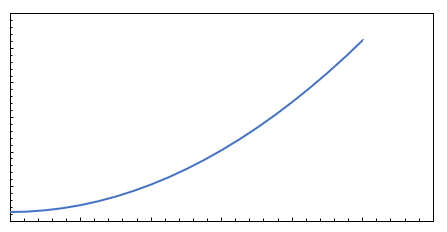
\includegraphics[scale=0.5]{t2.PNG}
        \caption{Imagem importada no Exemplo 1.}
        \label{fig:ex1_1}
    \end{figure}
    
    Os parâmetros utilizados na clusterização são $eps=0.15$ e $p\_min=25$. Os clusters obtidos pelo DBSCAN são ilustrados na Fig. \ref{fig:ex1_2}. Vale citar que os valores máximos dos eixos $x$ e $y$ são, respectivamente, 15 e 120. Estes valores também devem ser informados pelo usuário.
    
    \begin{figure}[h]
        \centering
        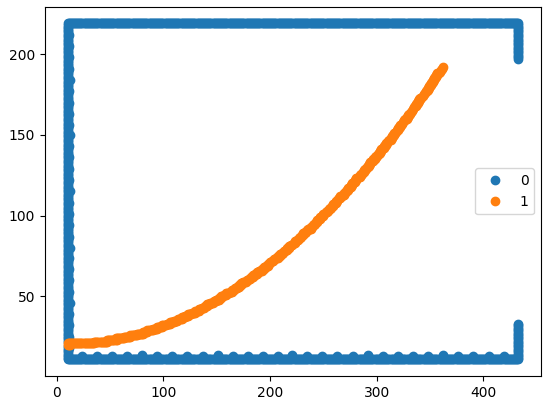
\includegraphics[scale=0.4]{clusters_ex1.PNG}
        \caption{Cluster obtidos no Exemplo 1.}
        \label{fig:ex1_2}
    \end{figure}
    
    Assim, o usuário seta que o grupo 0 são os eixos $xy$ e o grupo 1 é a série desejada. A Fig. \ref{fig:ex1_3} ilustra os resultados obtidos pela clusterização (pontos da série ``Clusterizado'') em comparação com o gráfico original (série ``y\_analtico'').
    
    Pode-se concluir a partir da Fig. \ref{fig:ex1_3} que os resultados obtidos pelo algorítmo foram excelentes em relação a referência. Todos os pontos calculados caíram exatamente em cima da série original, conforme o esperado.
    
    \begin{figure}[H]
        \centering
        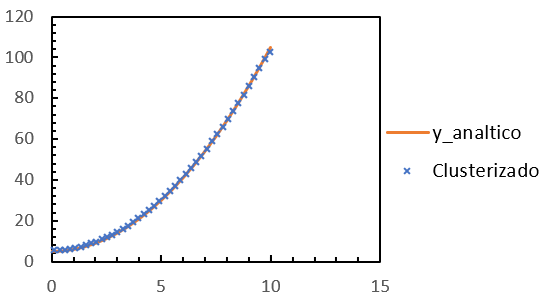
\includegraphics[scale=0.55]{ex1_results.PNG}
        \caption{Resultados obtidos no Exemplo 1.}
        \label{fig:ex1_3}
    \end{figure}
    
    % **************************************************************************
    \subsection{Exemplo 2: Gráfico com múltiplas séries}    
    % **************************************************************************
    
    No segundo exemplo é gerado um gráfico no Excel com três diferentes séries que representam as seguintes funções:
    
    \begin{itemize}
        \item $f_1(x)=100x+10$, com $0\leq x \leq 15$
        \item $f_2(x)=x^3$, com $0\leq x \leq 15$
        \item $f_3(x)=1000\sin{x}+500x$, com $1\leq x \leq 15$
    \end{itemize}
    
    A imagem importada pelo código é ilustrada na Fig. \ref{fig:ex2_1}.
    
    \begin{figure}[h]
        \centering
        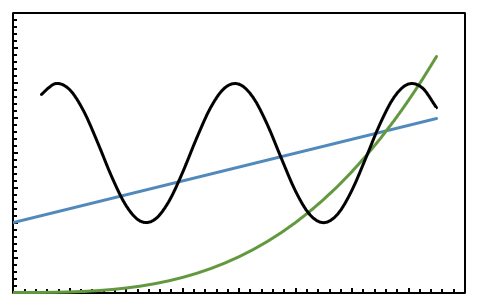
\includegraphics[scale=0.5]{t4.PNG}
        \caption{Imagem importada no Exemplo 2.}
        \label{fig:ex2_1}
    \end{figure}
    
    Os parâmetros utilizados na clusterização deste exemplo são os mesmos do primeiro exemplo ($eps=0.15$ e $p\_min=25$). Os clusters obtidos pelo DBSCAN são ilustrados na Fig. \ref{fig:ex2_2}. Vale citar que os valores máximos dos eixos $x$ e $y$ foram informados manualmente pelo usuário.
    
    \begin{figure}[h]
        \centering
        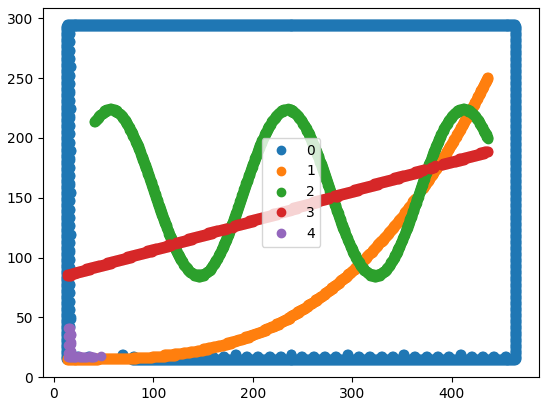
\includegraphics[scale=0.4]{cluster_ex2.PNG}
        \caption{Clusters obtidos no Exemplo 2.}
        \label{fig:ex2_2}
    \end{figure}
    
    Com base na Fig. \ref{fig:ex2_2}, o usuário deve informar que os clusters 0 e 4 correspondem aos eixos $xy$, enquanto que os clusters 1, 2 e 3 são séries desejadas. Assim, os resultados obtidos pelo algoritmo são ilustrados na Fig. \ref{fig:ex2_3} através das séries ``Cluster Serie\_1'', ``Cluster Serie\_2'' e ``Cluster Serie\_3'' no gráfico.
    
    A Fig. \ref{fig:ex2_3} permite concluir que os resultados deste exemplo foram também satisfatório. Todos os pontos obtidos para as três séries coincidiram exatamente com as funções analíticas originais. Vale observar ainda que, mesmo existindo o cruzamento entre linhas de diferentes séries em diversos pontos, o algoritmo foi capaz de contornar essa dificuldade e o resultado não foi afetado.
    
    \begin{figure}[h]
        \centering
        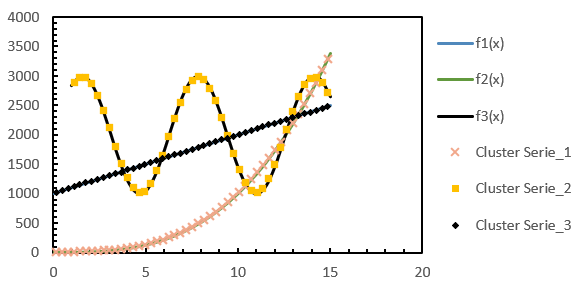
\includegraphics[scale=0.6]{ex2_results.PNG}
        \caption{Resultados obtidos no Exemplo 2.}
        \label{fig:ex2_3}
    \end{figure}
    
    % **************************************************************************
    \section{Conclusão}
    % **************************************************************************
    
    Os resultados apresentados concluem que o algoritmo desenvolvido nesse projeto cumpriu satisfatoriamente seu objetivo de obter automaticamente os pontos de séries de um gráfico a partir da imagem em PNG. Ambos os exemplos encontraram convergência facilmente do DBSCAN utilizando os mesmos parâmetros. O algoritmo se mostrou ainda robusto ao conseguir trabalhar com diversas séries no mesmo gráfico e que contem cruzamentos entre diferentes linhas. 
    
    Obviamente o algoritmo desenvolvido possui uma série de limitações que poderiam ser atacadas em oportunidades futuras. Como limitações e hipóteses simplificadoras assumidas, destacam-se:
    
    \begin{itemize}
        \item A necessidade do usuário informar quais os clusters se referem aos eixos $xy$ do gráfico para que estes sejam excluídos da resposta final. Esta tarefa poderia ser realizada automaticamente pelo código ao buscar por relações matemáticas entre os valores $\bar{y}_i$ obtidos pelos clusters que indicassem qual deles se refere aos eixos;
        
        \item A necessidade do usuário informar os valores máximos dos eixos, considerando que ambos iniciam no zero. Um algoritmo de identificação de números na imagem poderia ser aplicado para identificar esses valores, permitindo que o PNG inicial contivesse os labels dos eixos;
        
        \item A dificuldade em lidar com gráficos que possuam legenda dentro da área de plotagem. Essa limitação poderia ser contornada ao programar funções que permitissem identificar no PNG a área da legenda e retirar os pixels referentes à ela da clusterização.
        
    \end{itemize}
    
    Assim, conclui-se que este trabalho aplica com sucesso uma técnica não supervisionada de Machine learning em uma aplicação gráfica. O projeto final encontra-se com algumas limitações e hipóteses simplificadoras, porém este se mostra robusto e com bastante potencial. Tais limitações poderiam ser vencidas futuramente, caso haja interesse no desenvolvimento mais profundo deste projeto.
    
    % ``I always thought something was fundamentally wrong with the universe'' \citep{adams1995hitchhiker}
    
    % \bibliographystyle{plain}
    % \bibliography{references}
\end{document}
